\documentclass{article}

\usepackage{graphicx}
\usepackage{tikz}
\usepackage{tikzsymbols}
\usetikzlibrary{calc,patterns,shapes.geometric}
\pagestyle{empty}
\usepackage[margin=0pt]{geometry}
\geometry{papersize={14in,12in}}

\def\centerarc[#1](#2)(#3:#4:#5){\draw[#1] ($(#2)+({#5*cos(#3)},{#5*sin(#3)})$) arc (#3:#4:#5);}

\begin{document}
	\begin{figure}
		\centering
		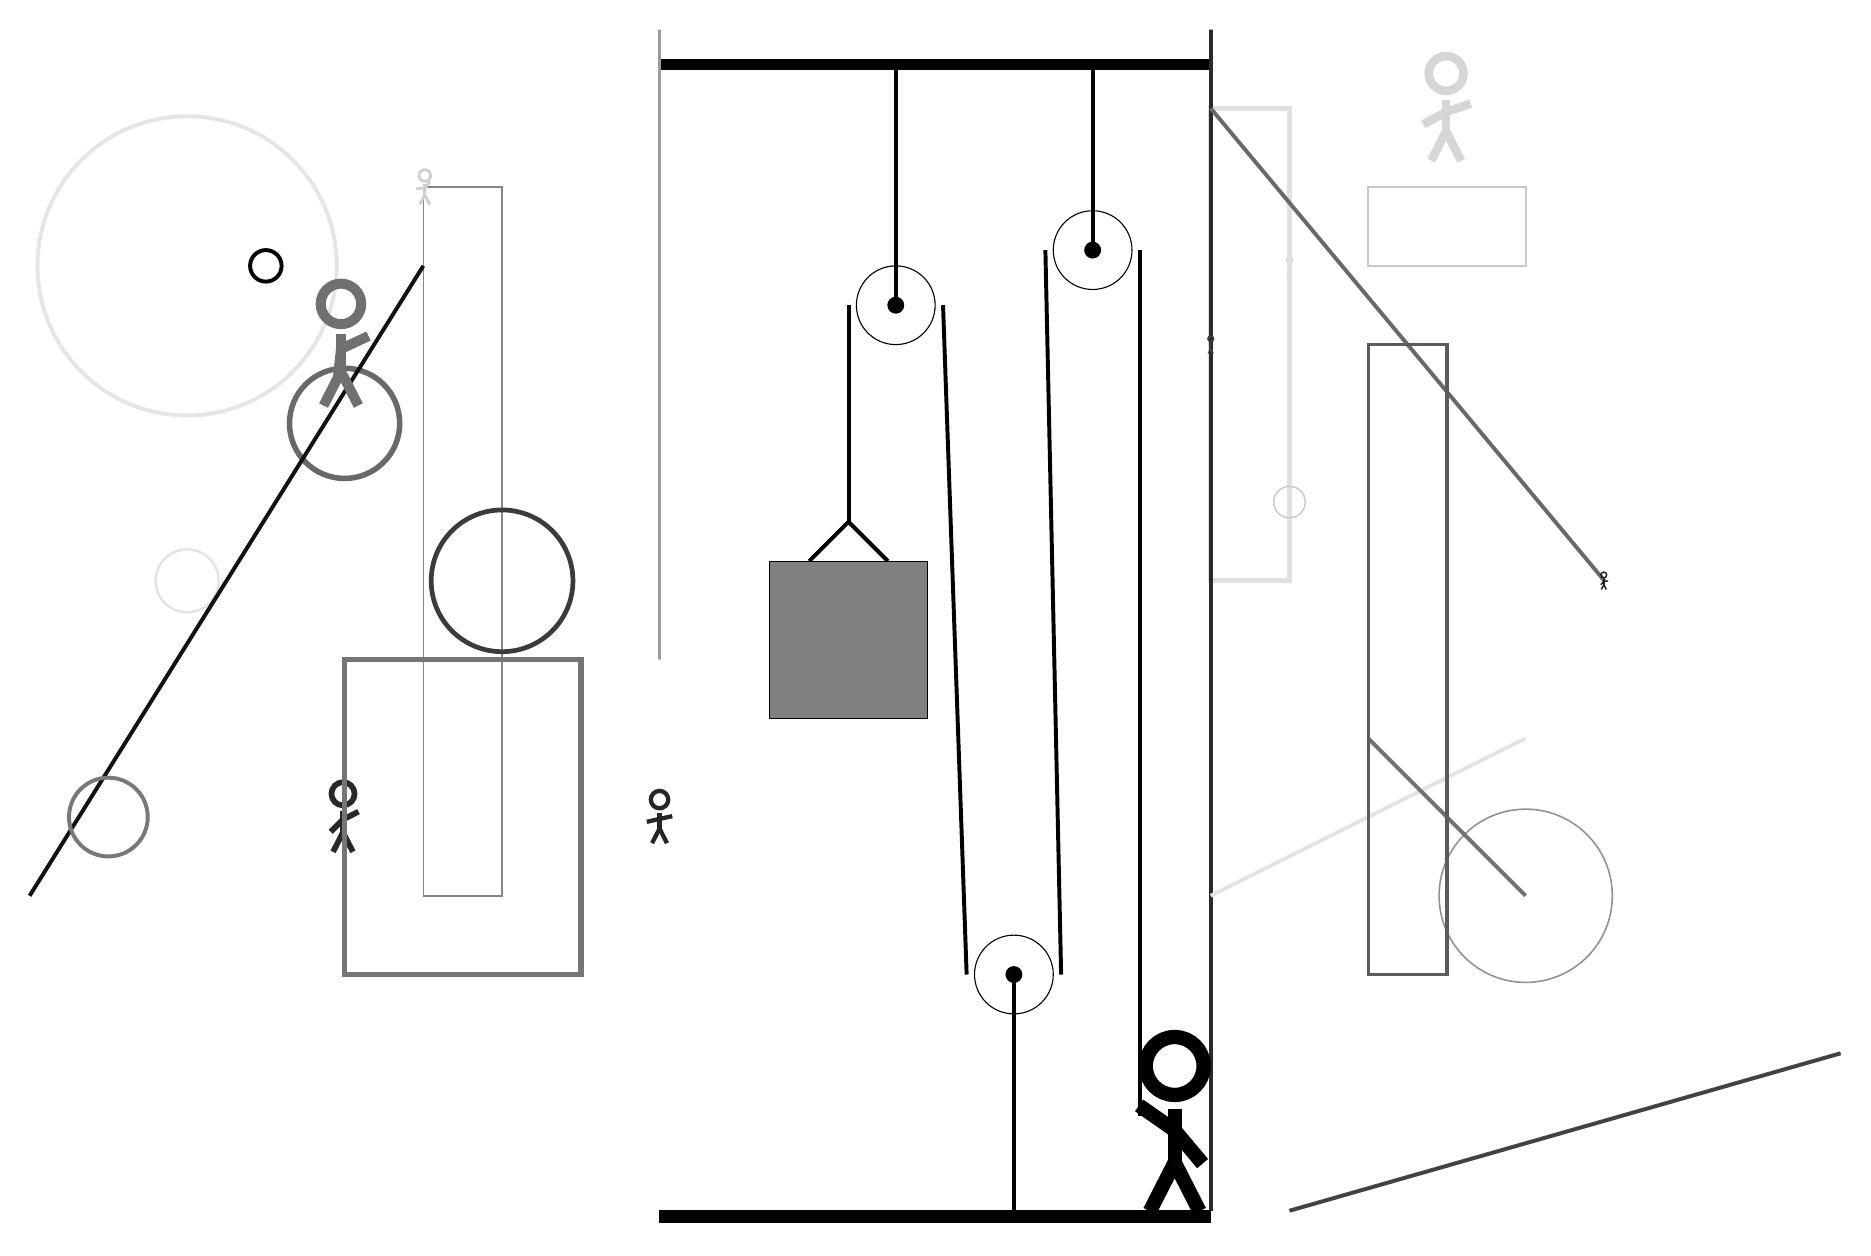
\begin{tikzpicture}
			%%%%% START %%%%%
			
			\draw[fill=black] (-2, 11.5) rectangle (5, 11.625);
			
			\draw (1, 8.5) circle (0.5);
			\draw[fill=black] (1, 8.5) circle (0.1);
			\draw[line width=0.5mm]  (1, 11.5) -- (1, 8.5);
			
			\draw[fill=white](2.5, 0.0) circle (0.5);
			\draw[fill=black] (2.5, 0.0) circle (0.1);
			\draw[line width=0.5mm]  (2.5, -3) -- (2.5, 0.0);
			
			\draw[fill=white](3.5, 9.2) circle (0.5);
			\draw[fill=black] (3.5, 9.2) circle (0.1);
			\draw[line width=0.5mm] (3.5, 11.5) -- (3.5, 9.2);
			
			\node[line width=0.7mm, color=black!22] at (6, 9) {\Strichmaxerl[1][68][89]};
			
			\draw[line width=0.5mm, color=black!75](5, 11) -- (5, -3);
			\draw [line width=0.5mm, color=black!10](-8, 9) circle (1.9);
			\draw[line width=0.6mm, color=black!12] (6, 11) rectangle (5, 5);
			\draw[line width=0.5mm, color=black!74](6, -3) -- (13, -1);
			\node[line width=0.3mm, color=black!84] at (-6, 2) {\Strichmaxerl[4][45][27]};
			
			\draw[line width=0.5mm, color=black!84] (5, 12) rectangle (5, -3);
			\draw[line width=0.5mm, color=black!11](5, 1) -- (9, 3);
			\draw [line width=0.3mm, color=black!11](-8, 5) circle (0.4);
			\node[line width=0.2mm, color=black!16] at (8, 11) {\Strichmaxerl[6][28][19]};
			\draw [line width=0.5mm, color=black!98](-7, 9) circle (0.2);
			\draw [line width=0.2mm, color=black!43](9, 1) circle (1.1);
			\draw[line width=0.5mm, color=black!56](7, 3) -- (9, 1);
			
			\draw[line width=0.2mm, color=black!47] (-4, 10) rectangle (-5, 1);
			\node[line width=0.5mm, color=black!19] at (-5, 10) {\Strichmaxerl[2][3][52]};
			\node[line width=0.4mm, color=black!85] at (-2, 2) {\Strichmaxerl[3][13][12]};
			
			\draw[line width=0.5mm, color=black!59](10, 5) -- (5, 11);
			\draw[line width=0.4mm, color=black!64] (7, 0) rectangle (8, 8);
			\draw[line width=0.3mm, color=black!21] (7, 9) rectangle (9, 10);
			\draw [line width=0.7mm, color=black!59](-6, 7) circle (0.7);
			\draw[line width=0.5mm, color=black!93](-5, 9) -- (-10, 1);
			\node[line width=0.6mm, color=black!56] at (-6, 8) {\Strichmaxerl[7][84][25]};
			
			\draw [line width=0.6mm, color=black!77](-4, 5) circle (0.9);
			\draw [line width=0.5mm, color=black!53](-9, 2) circle (0.5);
			\draw[line width=0.7mm, color=black!54] (-3, 0) rectangle (-6, 4);
			\draw [line width=0.2mm, color=black!20](6, 6) circle (0.2);
			\node[line width=0.5mm, color=black!75] at (5, 8) {\Strichmaxerl[1][74][85]};
			\node[line width=0.4mm, color=black!88] at (10, 5) {\Strichmaxerl[1][45][7]};
			
			\draw[line width=0.4mm, color=black!39] (-2, 12) rectangle (-2, 4);
			
			\draw[line width=0.5mm] (-0.1, 5.25) -- (0.4, 5.75) -- (0.9, 5.25);
			\draw[fill=black!50] (-0.6, 5.25) rectangle (1.4, 3.25);
			
			\draw[line width=0.5mm] (0.4, 8.5) -- (0.4, 5.75);
			\centerarc[line width=0.5mm](1, 8.5)(0:180:0.6);
			\draw[line width=0.5mm](1.6, 8.5) -- (1.9, 0.0);
			\centerarc[line width=0.5mm](2.5, 0.0)(180:360:0.6);
			\draw[line width=0.5mm](3.1, 0.0) -- (2.9, 9.2);
			\centerarc[line width=0.5mm](3.5, 9.2)(0:180:0.6);
			\draw[line width=0.5mm](4.1, 9.2) -- (4.1, -1.8);
			
			\node at (4.5, -1.9) {\Strichmaxerl[10][-35][-50]};
			
			\draw[fill=black] (-2, -3) rectangle (5, -3.15);
			
			%%%%% END %%%%%
		\end{tikzpicture}
	\end{figure}	
\end{document}